\chapter{Optimizing patients travel}

\section{Context}

Cancer treatment delay is a problem in health systems worldwide, increasing
mortality for many types of cancers \cite{hanna_mortality_2020}, including
breast cancer \cite{caplan_delay_1992, williams_assessment_2015,
    pace_delays_2015}. Distance between patients residence and diagnosing hospitals
is among the factors causing these delays, especially for cancer types that are
hard to diagnose \cite{flytkjaer_virgilsen_cancer_2019}. While accessibility to
healthcare is growing, research found that 8.9\% of the global population (646
million people) could not reach healthcare within one hour if they had access to
motorized transport \cite{weiss_global_2020}. Thus, a non insignificant part of
the population might be exposed to lower prognosis.

The benefits of centralized healthcare have been debated. A centralized approach
often requires patients to travel far away from their home and their local
community hospitals \cite{woo_centralisation_2012}. Patients subject to longer
travels to reach a specialized hospital are likely to be affected by the travel
burden and separation from their social environment \cite{payne_impact_2000}. In
the debate between local versus centralized healthcare provision, there are
evidence of an association between travel distance and health outcomes
\cite{kelly_are_2016}. Unsurprisingly, travel to cancer treatment is
inconvenient for some patients and might even act as a barrier to treatment
\cite{payne_impact_2000}. Research also showed that patients who lived far from
hospitals and had to travel more than 50 miles had a more advanced stage at
diagnosis, lower adherence to encoded treatments, a worse prognosis, and a worse
quality of life \cite{ambroggi_distance_2015}. More research linked travel
burden with lower treatment compliance
\cite{dutta_evaluation_2013,guidry_transportation_1997}. The distance from the
hospital influences the choice of appropriate treatment by cancer patients. In
breast cancer, patients living farther from a radiation treatment facility more
often underwent mastectomy instead of breast conservative surgery
\cite{schroen_impact_2005,celaya_travel_2006,voti_treatment_2006,meden_relationship_2002,nattinger_relationship_2001,boscoe_geographic_2011}
or did not undergo radiotherapy after breast cancer surgery
\cite{satasivam_dilemma_2014,schroen_impact_2005,celaya_travel_2006}. In non
small cell lung cancer, patients were most likely to not undergo potentially
curative surgery if they lived far from a specialist hospital and only attended
a general hospital for their care \cite{tracey_patients_2015}. Moreover, the
necessity for repeated visits for cancer diagnosis and treatment makes distance
an even more important issue for the patient\cite{guidry_transportation_1997}.
However, for hard to diagnose cancer type like rectum or testis cancers,
distance was associated with decreasing odds of advanced disease stage
\cite{virgilsen_travel_2019}. This is possibly due to being treated in more
specialized hospitals. The negative effects of centralized healthcare are even
more pronounced for patients living in rural areas. Indeed, rural cancer
patients face more challenges in receiving care, due to the limited availability
of providers and clinical trials, as well as transportation barriers and
financial issues \cite{charlton_challenges_2015}. There are evidence of poorer
treatments and outcomes for patients living in rural areas. For instance, in
Australia, poorer survival and variations in clinical management have been
reported for breast cancer women living in non metropolitan areas
\cite{dasgupta_variations_2018}. Still in Australia, breast cancer women treated
in a rural hospital had a reduced likelihood of breast conservative surgery
\cite{hall_unequal_2004}.  The hazard of death from ovarian cancer was greater
in women treated at a public general hospital than in women treated at a
gynecological oncology service \cite{tracey_effects_2014}. Contacting a
provincial hospital instead of a university hospital might lead to diagnosis and
treatment delays, which could be improved by a better referral system
\cite{thongsuksai_delay_2000}. In Australia, patients living farther from a
radiotherapy service were more likely to die of rectal cancer, with a 6\% risk
increase for each additional 100km \cite{baade_distance_2011}. In Rwanda, rural
breast cancer patients who lived in the same district as breast cancer hospitals
had a decreased likelihood of system delay \cite{pace_delays_2015}. In Canada,
place of residence seems to influence health outcomes in patients with diffuse
large B-cell lymphoma \cite{lee_effect_2014}. They found that rural and
metropolitan patients had similar survival; however, patients in small and
medium urban areas experienced worse outcomes than those in metropolitan areas.
Thus, rural culture might have a dual effect on health outcomes. On one hand,
distance, transportation, and health services shortage are barriers to
healthcare. On the other hand, rural culture comes with community belonging, and
deeper relationship with health care professionals, which might be beneficial
for some patients \cite{brundisini_chronic_2013}.

Additionally to having a negative impact on patients health, longer travels
participate in global warming due to their \ac{co2} emissions.  The World Health
Organization called climate change the greatest threat to global health in the
21st century, significantly affecting hundreds of millions of people
\cite{change_climate_2015}. The United Nations created the \ac{ipcc} to assess
the science related to climate change and provide governments with scientific
information that they can use to develop climate policies. The health care
sector is an important contributor to \ac{co2} emissions. An international
comparison of health care carbon footprints showed that, on average, the health
carbon footprint in 2014 constituted 5.5\% of the total national carbon
footprint \cite{pichler_international_2019}. Hence, the health sector has a
responsibility to take climate action
\cite{health_care_without_harm_hcwh_global_2021}. Especially since the Paris
Agreement, where countries agreed to cut \ac{ghg} emissions to keep global
warming below 2 degrees Celsius. Today, hospitals are powered by fossile energy
such as coal, oil and gas. Healthcare related travels, and the manufacture and
transport of healthcare products are also major causes of \ac{ghg} emissions.
Ultimately, all health systems will need to reach near zero emissions by 2050,
which can be more cost effective than business as usual. The Lancet Countdown on
health and climate change started to review annually the relation between health
and climate change \cite{watts_2020_2021}. A large share of these carbon
emissions is due to patients journeys
\cite{andrews_carbon_2013,nicolet_what_2022} because most patients travel by car
\cite{forner_carbon_2021}. With centralization of care, patients are encouraged
to be treated in large hospitals for better outcome \cite{eskander_health_2016}.
Such hospitals are in urban areas, and the populations living in rural areas
will have to travel longer to reach these centers, resulting in higher carbon
emissions. In France, few studies have evaluated the ecological impact of cancer
care \cite{guillon_empreinte_2020}. The Shift Project is a French think tank
that works towards a carbon-free economy. As a non-profit organization, they
inform and influence the debate on the energy transition. In 2021, the Shift
Project released a report on how to decarbonize the health care sector in France
\cite{the_shift_project_plan_2021}. They identified that most of the \ac{ghg}
emissions were scope 3 emissions, which are indirect emissions that occur in the
hospitals value chain. Among these emissions, the largest source are
pharmaceuticals and medical device buying, followed by patients and visitors
transportation. The Shift Project states that emissions related to
transportation should be cut by 99\%, through measures like increasing public
transportation and telemedicine.Telemedicine includes all medical practices that
allow patients to be treated remotely from a health facility. It has been used
increasingly around the world, even in oncology where it is sometimes referred
as teleoncology
\cite{mooi_teleoncology_2012,sabesan_are_2014,sabesan_timely_2014,sabesan_medical_2014}.
Teleoncology models have been used to provide access to specialized cancer care
for people in rural, remote and other disadvantaged areas, which minimizes the
access difficulties and disparities \cite{sabesan_telemedicine_2012,
    sabesan_are_2014}. Teleoncology models can also be beneficial in training
medical, nursing, and allied health trainees and staff at rural centers
\cite{sabesan_medical_2014}. Research reported multiple benefits of telemedicine
at every level of care, including education, prevention, diagnosis, treatment,
and monitoring \cite{bertucci_outpatient_2019}. However, besides the expected
benefits, several questions and fears are emerging
\cite{bertucci_outpatient_2019}. First, there is a risk of patient isolation,
due to the absence of in-person meeting. It is also more difficult to build an
atmosphere of trust during remote consultations and the examinations might be of
inferior quality. Finally, digital divide is a major limitation of e-health, as
certain categories of patients do not have access to the internet or to a
smartphone.

In this chapter, we analyzed the travels of cancer patients in metropolitan
France. Our goal was to assess whether the earlier observations on the negative
effects of centralization of care were happening in France. Hence, we first
described the travel duration distribution in metropolitan France, and compared
it with the population densities and the oncology specialization of the visited
hospital. Then, we argued that the negative effects of travel on cancer patients
was not only due to driving distance and duration: the road sinuosity should
also be taken into account. We proposed a travel burden index, which is a
composite indicator based on multiple variables to evaluate how easy it is to go
from a population location to an hospital. Additionally, we estimated the carbon
footprint of cancer patients travels, and compared these numbers across the
different regions. Finally, we ran an optimization algorithm to simulate the
scenario where every patient traveled to the closest hospital, such that the
hospitals capacities were not exceeded. We only considered Breast Cancer
patients as this cancer is relatively frequent, and many hospitals have the
required expertise.

\section{Methods}

\subsection{Travel burden index}

In this section, we detail our method for computing the travel burden score. We
used the \ac{pmsi} database to identify which hospitals were the patients
visiting from their population locations. We obtained 166,944 pairs of
population locations and hospitals. The number of distinct population locations
was 5,606, and the number of distinct hospitals was 978. We kept population
locations and hospitals located in metropolitan France only. From these pairs,
we retrieved routes from the Mapbox Directions API, with population locations as
starting point and hospitals as destinations.  We used driving car as the
default mean of transportation since most patients travel with personal car or
taxi to the hospital. The Mapbox API returns an array of routes ordered by
descending recommendation rank. We kept the first route for our analysis. From
this route, the overall duration and distance were returned directly by the API.
Addition-ally, we extracted more variables: the number of roundabouts and the
road sinuosity. The road sinuosity was computed as the ratio between the GPS
distance and straight distance. The sinuosity is 1 for perfectly straight roads
and increases with the number of turns. We computed this ratio for every road
leg and summed them up to obtain the overall road sinuosity. We apply standard
scaling (0 mean, unit variance) on these 4 variables, and we ran a \ac{pca} on
top of the scaled data. We used the first PCA component as our score.

\subsection{Carbon footprint estimation}

We now explain how we estimated the \ac{co2} emissions from a driving route. We
only consider the direct emissions, proportional to the traveled distance and
car fuel consumption. As mentioned earlier, we extracted the GPS routes between
population locations and hospitals. For each pair of locations, we have the
number of patients and number of individual stays. We use the number of stays as
number of travels between population locations and hospitals. We stored the
overall distance extracted from the Mapbox API for each route. However, we do
not know which car was used by patients during their visit to the hospital.
Instead, the average \ac{co2} emission rate obtained from the French Agency for
the Environment and Energy Management (ADEME) to estimate the emissions.
Emissions were computed for every pair of population locations and hospitals, as
the product between the number of patients stays, the GPS distance and the
average \ac{co2} emission rate. In 2018, the average emission rate was 112 grams
of \ac{co2} per kilometer. We should mention that the 2018 average emission rate
is calculated from the new cars sold that year. The average emission rates for
the previous years are available on the ADEME website. There is a downward
trend, but the number was roughly stable between 2014 and 2019, ranging from 114
g\ac{co2}/km to 112 g\ac{co2}/km. Even though the 2018 average emissions might not
perfectly fit to the actual distribution, we believe that this estimator will be
good enough for our analysis.

\subsection{Routing optimization}

Finally, we detail in this section the methodology we used for optimizing the
patients travel. We focused on breast cancer patients only, since there are
many hospitals capable of treating this pathology. Since we do not have
very precise informations on the patients conditions, we chose to optimize
for a simple metric: travel distance. The idea was to simulate what would
happen if every patient traveled to the closest specialized hospital, while
making sure the hospitals capacities were not exceeded. We modeled this problem
as an \acf{ot} task. In the following paragraphs, we first introduce what is
\ac{ot}, and then explained how we applied it to our problem.

\acf{ot} is the study of the optimal transportation and allocation of resources.
It was introduced in 1781 by the French mathematician Gaspard Monge,
\cite{monge_memoire_1781} who was interested in the problem of the optimal way
of redistributing mass. The problem was, given a pile of soil, how can it be
transported and reshaped to form an embankment with minimal effort ? During
the World War II, the soviet mathematician Leonid Kantorovitch brought major
advances in the field \cite{kantorovitch_translocation_1958}, by allowing the
mass to be split during transportation. A couple of years later, George
Dantzig introduced the Simplex Algorithm to solve Linear Programs, including
the Kantorovitch Problem. However, solving this Linear Program becomes
untractable whenever the dimension is large. In the recent years, an
entropic regularization term was added to the \ac{ot} formulation, allowing to
find the optimum in a very fast way \cite{cuturi_sinkhorn_2013}, using the
Sinkhorn-Knopp's algorithm \cite{knopp_concerning_1967}.

We now explain more formally how to solve the \ac{ot} problem with entropic
regularization. Consider two distributions $\alpha$ and $\beta$, with
respectively $n$ and $m$ points $x$ and $y$, each associated with positive weights
$a_i$ and $b_j$ such that $\sum_{i=1}^{n} a_i = \sum_{j=1}^{m} b_i = 1$. The
displacement of mass between the two distributions can be described by a
set of transport plan, or couplings, defined on \cref{eq:couplings}. In
this equation, the couplings $U(a, b)$ are the set of transport plan
$P \in \mathbb{R}_{+}^{n \times m}$, that satisfies the transportation of mass
constraints $P \mathbf{1}_m = a, P^T \mathbf{1}_n = b$. Intuitively, all
the mass from the first distribution should be moved to the second
distribution. Thus, summing on $P$ column-wise or row-wise should return $a$
and $b$. We seek to find the transport plan $P \in U(a, b)$ that minimizes the
cost \cref{eq:ot-min}. The first term in this cost is the distance $d(x_i, y_j)^p$ between
the two points $x_i$ and $y_j$. The next term is the Entropic Regularization,
weighted by $\epsilon$. The lower $\epsilon$ is, the closer we get to the
non-regularized \ac{ot} problem. The minimum solution can be obtained
with the Sinkhorn-Knopp's algorithm \cite{knopp_concerning_1967}, as
explained in \cite{peyre_computational_2020,cuturi_sinkhorn_2013}. The output
of the algorithm is the optimal transport plan $\sigma^*$, that moves the input
distribution to the output distribution in the most cost effective way.

\begin{equation}
    U(a, b) = \lbrace P \in \mathbb{R}_{+}^{n \times m} ; P \mathbf{1}_m = a, P^T \mathbf{1}_n = b \rbrace
    \label{eq:couplings}
\end{equation}

\begin{equation}
    \underset{P \in U(a, b)}{min} \sum_{i,j} d(x_i, y_j)^p P_{i,j} + \sigma P_{i,j} log(\frac{P_{i,j}}{a_i b_j})
    \label{eq:ot-min}
\end{equation}

In our case, we want to find the optimal way to move patients from their
$n$ population locations, to the $m$ hospitals. The distance metric
$d(x_i, y_j)$ is the driving distance between the municipality $i$ and the
hospital $j$. The weights $a$ and $b$ correspond to the populations and
hospitals capacities respectively. We normalized the populations and capacities
so that $a$ and $b$ sum to one. Thus, $a_i$ corresponds to the proportion of
patients living in municipality $i$, and $b_j$ to the proportion of patients
that the hospital $j$ can host. The $\sigma^*$ output matrix contains the
overall proportions of patients sent from the municipality $i$ to the
hospital $j$. We multiply each element in this matrix by the total number of
patients, and round the result to get the number of patients traveling from
the municipality to the hospital.

\section{Results}

\subsection{Patients travel description}

We included 493,526 travels for 12 cancer types, treated in 978 distinct
hospitals as summarized in \cref{table:distance_and_co2}.

\begin{table}[h]
    \centering
    \resizebox{\textwidth}{!}{%
        \begin{tabular}{|l|r|r|r|r|r|r|r|}
            \hline
            % Headers
            ~                                                                                & \textbf{N stays} & \textbf{Median duration} & \textbf{Median distance} & \textbf{Total distance} & \textbf{N Hospitals} & \textbf{\% Hospitals} & \textbf{\ac{co2} Emissions} \\ \hline
            % Pathology
            \multicolumn{8}{|l|}{\textbf{Cancer type}}                                                                                                                                                                                                                       \\ \hline
            Malignant melanoma and other malignant skin tumors                               & 104,429          & 21.56                    & 16.18                    & 3,214,375.72            & 894                  & 91\%                  & 360.01                      \\ \hline
            Malignant tumors of the eye, brain and other parts of the central nervous system & 7,904            & 44.39                    & 44.43                    & 616,675.46              & 327                  & 33\%                  & 69.07                       \\ \hline
            Malignant tumors of the lip, oral cavity and pharynx                             & 13,115           & 29.55                    & 26.35                    & 629,616.37              & 659                  & 67\%                  & 70.52                       \\ \hline
            Malignant tumors of the thyroid and other endocrine glands                       & 9,059            & 27.57                    & 22.68                    & 405,445.77              & 564                  & 58\%                  & 45.41                       \\ \hline
            Malignant tumors of the digestive organs                                         & 81,440           & 24.31                    & 20.18                    & 3,330,910.43            & 858                  & 88\%                  & 373.06                      \\ \hline
            Malignant tumors of the male genital organs                                      & 47,472           & 24.68                    & 20.66                    & 1,869,128.99            & 815                  & 83\%                  & 209.34                      \\ \hline
            Malignant tumors of the female genital organs                                    & 29,501           & 25.75                    & 21.48                    & 1,249,403.48            & 799                  & 82\%                  & 139.93                      \\ \hline
            Malignant tumors of the respiratory and intrathoracic organs                     & 30,228           & 31.71                    & 28.69                    & 1,523,374.66            & 758                  & 78\%                  & 170.62                      \\ \hline
            Malignant tumors of bone and articular cartilage                                 & 2,452            & 41.80                    & 39.32                    & 180,105.78              & 323                  & 33\%                  & 20.17                       \\ \hline
            Malignant tumors of the urinary tract                                            & 75,140           & 22.74                    & 17.90                    & 2,565,232.46            & 803                  & 82\%                  & 287.31                      \\ \hline
            Malignant breast tumors                                                          & 86,237           & 24.94                    & 20.26                    & 3,290,349.47            & 810                  & 83\%                  & 368.52                      \\ \hline
            Malignant tumors of mesothelial tissue and soft tissue                           & 6,549            & 33.35                    & 30.04                    & 402,222.65              & 677                  & 69\%                  & 45.05                       \\ \hline
            % Cluster
            \multicolumn{8}{|l|}{\textbf{Hospital Cluster}}                                                                                                                                                                                                                  \\ \hline
            Cluster 1                                                                        & 121,890          & 33.33                    & 29.73                    & 6,586,967,47            & 79                   & 8\%                   & 737.74                      \\ \hline
            Cluster 2                                                                        & 38,606           & 24.46                    & 21.35                    & 1,630,935,96            & 39                   & 4\%                   & 182.66                      \\ \hline
            Cluster 3                                                                        & 244,493          & 22.73                    & 18.03                    & 8,377,446,27            & 451                  & 46\%                  & 938.27                      \\ \hline
            Cluster 4                                                                        & 86,245           & 21.32                    & 16.22                    & 2,634,153,25            & 348                  & 36\%                  & 295.03                      \\ \hline
            Cluster 5                                                                        & 7                & 15.13                    & 12.17                    & 137.79                  & 2                    & 0\%                   & 0.02                        \\ \hline
            Cluster 6                                                                        & 13               & 30.13                    & 31.55                    & 440.41                  & 3                    & 0\%                   & 0.05                        \\ \hline
            Cluster 8                                                                        & 2,272            & 18.43                    & 11.55                    & 467,60.09               & 56                   & 6\%                   & 5.24                        \\ \hline
        \end{tabular}
    } \caption{ \textbf{Patients travel description for each pathology.} We
        included 493,526 travels for 12 cancer types, treated in 978 distinct
        hospitals. For each pathology, we compared the median travel du-ration and
        median travel distance. For more frequent cancer types, the patients travel
        remain relatively short. However, for the less frequent tumors such as the
        eye, brain, and other parts of the central nervous system, the patients'
        travels were longer. This could probably be explained by the lower number of
        hospitals with the required specialization. We also looked at the travel
        duration based on the visited hospital. The patients' travels were longer
        when they visited more specialized hospitals from clusters 1 and 2. }
    \label{table:distance_and_co2}
\end{table}

The three most frequent pathologies were: malignant melanoma and other malignant
skin tumors (n=104,429 stays); malignant breast tumors (n=86,237 stays); and
malignant tumors of the digestive organs (n=81,440 stays). The rarest
pathologies were malignant tumors of the eye, brain, and other parts of the
central nervous system (n=7,904 stays); malignant tumors of mesothelial tissue
and soft tissue (n=6,549 stays); and malignant tumors of bone and articular
cartilage (n=2,452 stays). For each pathology, we compared the median travel
duration and median travel distance. For more frequent cancer types, the
patients travel remain relatively short, as there are many hospitals with the
required specialization. For instance, the shorter travels were for skin tumors
patients, with a median distance of 16.18 kilometers and a median duration of
21.56 minutes. Among all the hospitals included, 894 (91.4\%) of them performed
skin tumor surgeries. However, for the less frequent tumors such as the eye,
brain, and other parts of the central nervous system, the patients' travels were
longer. Indeed, the median travel duration was 41.8 minutes, and the median
distance was 39.32 kilometers. This could probably be explained by the lower
number of hospitals with the required specialization: only 323 (33\%) of them
performed such surgeries. We also looked at the travel duration based on the
visited hospital. To assess the oncology specialization of the hospitals, we
used the hospitals clusters defined in (63). Only the hospitals from clusters 1
to 4 can perform cancer surgeries. Hospitals from clusters 1 and 2 are the most
specialized oncology hospitals, with all the key services such as cancer
surgery, radiotherapy, and chemotherapy. They also have the largest surgeries
volumes and are often specialized in even the rarest cancer types. Such
hospitals are sparsely located, and often placed in large cities. The hospitals
from clusters 3 and 4 are less specialized and are in both large cities and
sub-urban areas. The patients' travels were longer when they visit more
specialized hospitals from clusters 1 and 2. This might be explained by either
the need for more specialized care, or by the reputation of the hospital and the
incentive of going there in-stead of a smaller but closer hospital. We are now
interested in the spatial distribution of the patients travel duration, in
metropolitan France. On \cref{fig:routes-duration-france}, we showed the average
driving duration per municipalities on a map (A). Municipalities are filled by
duration bins. Unsurprisingly, median travel duration is short-ed for patients
living in dense municipalities. The median duration for patients living in
municipalities with more than 200 inhabitants per km\textsuperscript{2} is 16.4
minutes. However, for patients living in municipalities with less than 30
inhabitants per km\textsuperscript{2}, the median duration is 50.7 minutes,
about three times higher. Most patients living in dense areas can reach
hospitals from the more specialized clusters in little time. However, travel
durations are highest for patients from rural areas reaching the most
specialized hospitals (C).

\begin{figure}[h!]
    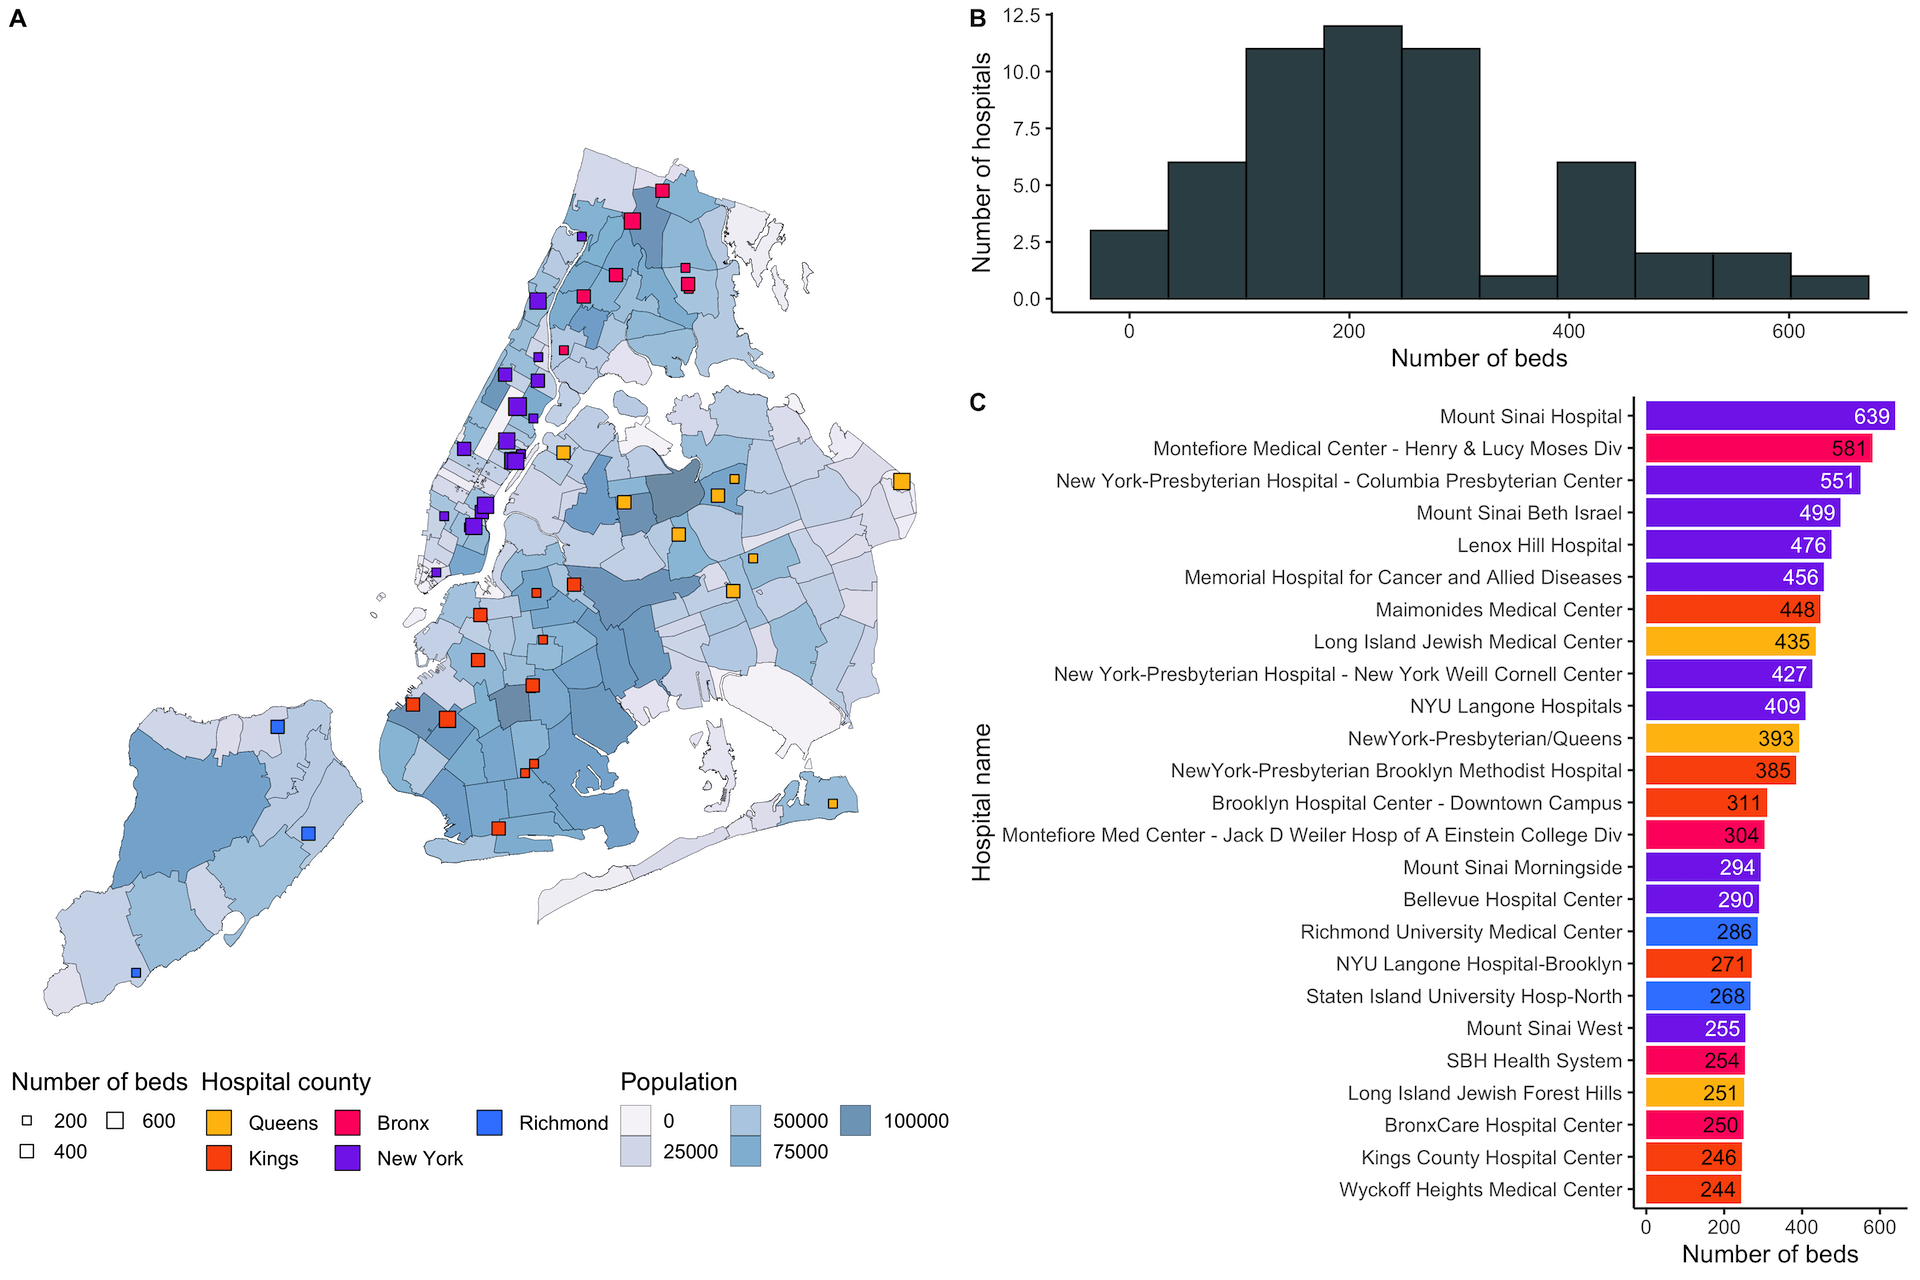
\includegraphics[width=0.9\textwidth]{images/routes/fig1.png}
    \centering
    \caption{ \textbf{Average driving duration for cancer patients in
            metropolitan France.} Map (A) displays the average driving duration by
        municipalities. The median travel duration is higher for municipalities
        with lower population densities (B). The median travel duration is
        especially high for patients from rural areas visiting specialized
        hospitals (C). Patients living in dense areas do not need to travel far
        when reaching specialized hospitals (C). }
    \label{fig:routes-duration-france}
\end{figure}

\subsection{Travel burden index}

While travel duration is a good proxy for the patients travel burden, it is not
the only contributor. In this section, we show the results of our travel burden
score. On \cref{fig:routes-burden-index}, map (A) shows the spatial distribution
of the travel burden score. We display the average travel burden score per
municipality. The lower the score, the lower the travel burden is. We
discretized the average score into 5 quantiles. For municipalities in the first
quantile, the average travel burden score is in the top 20\%, meaning that
patients travel are shorts and road sinuosity is low. The first quantile is
colored in dark green on the map. The last quantile is where travel burden score
is the highest, and these municipalities are colored in pale yellow.
Municipalities with lower population densities have a higher proportion of
routes with high travel burden. For instance, among all the municipalities with
population densities lower than 30 inhabitants per km\textsuperscript{2} 47.5\%
are in the worst quantile, compared to only 19.8\% for municipalities with 200
or more inhabitants per km\textsuperscript{2} (B). We now compare the travel
burden score with several variables, such as duration, distance, sinuosity,
number of roundabouts, as well as the road type ratio (C). As expected, higher
travel burden is associated with higher road sinuosity, distance, duration, as
well as higher number of roundabouts. The percentage of highway roads is also
the highest in this quantile.

\begin{figure}[h!]
    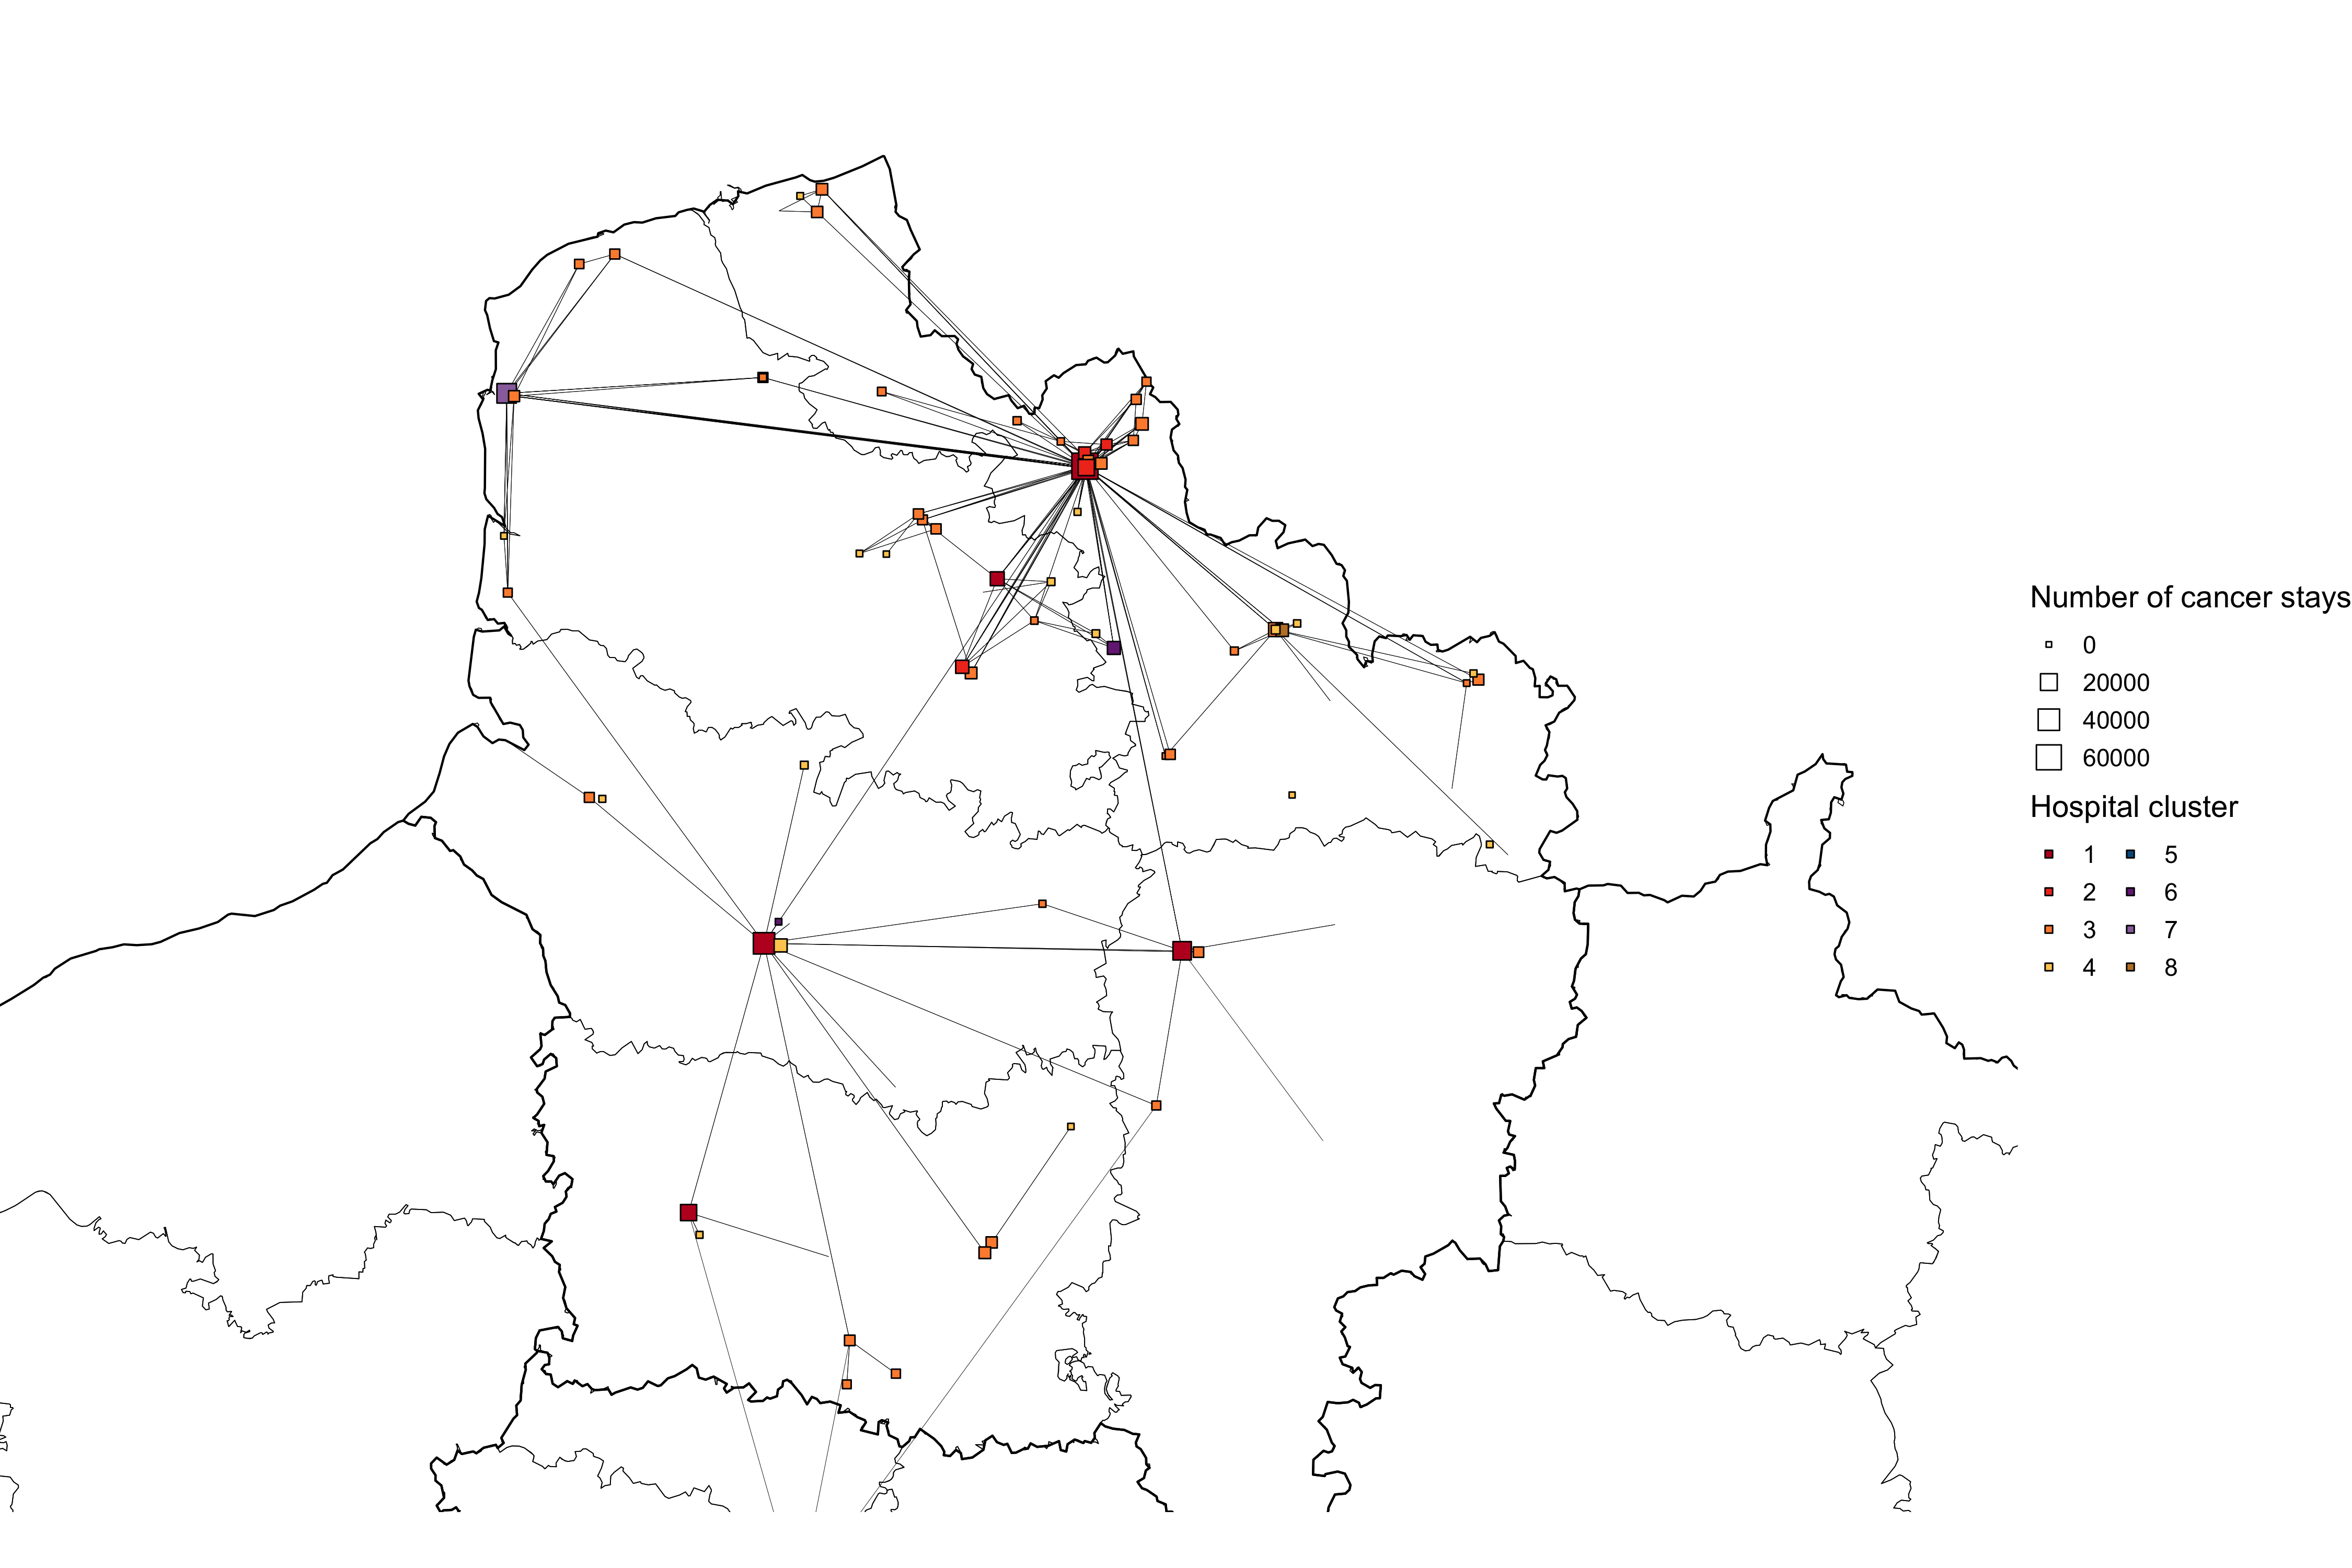
\includegraphics[width=0.9\textwidth]{images/routes/fig2.png}
    \centering
    \caption{
        \textbf{Travel burden index in metropolitan France.}
        The travel burden index is a composite score based on route duration,
        distance, number of roundabouts and sinuosity. The higher the score is,
        the more tedious the route is. The score distribution is displayed on
        map (A). The percentage of routes with higher scores increases in lower
        density areas (B). Figure (C) displays the input variables median values
        by score quantiles. For instance, the median road sinuosity is much
        higher when the score is high. }
    \label{fig:routes-burden-index}
\end{figure}

We focused on a single region, and compared the average travel burden score with
the main roads location, as illustrated on \cref{fig:travel-burden-paca}. We did
not show the roads that with were used by less than 5 patients during the year,
for clarity. In this region, we recall that the two largest cities are Marseille
and Nice, and that the accessibility is the highest along the coastline, where
the higher population densities are. The road network is the most developed on
the coastline, as well as around cities like Avignon and Gap. The areas that had
low accessibility scores have high travel burden scores, which makes sense since
the travel burden score was party computed with the travel duration to reach the
hospitals. However, we notice that some areas that had decent accessibility
scores can have average or high average travel burden scores. This is probably
due to the sinuosity of the roads, notably in the Var department, or in the
north of Nice city. The roads in these areas are often small, with a lot of
turns and roundabouts, increasing the travel tediousness. Overall, the travel
burden score is lower for municipalities near the main roads.

\begin{figure}[h!]
    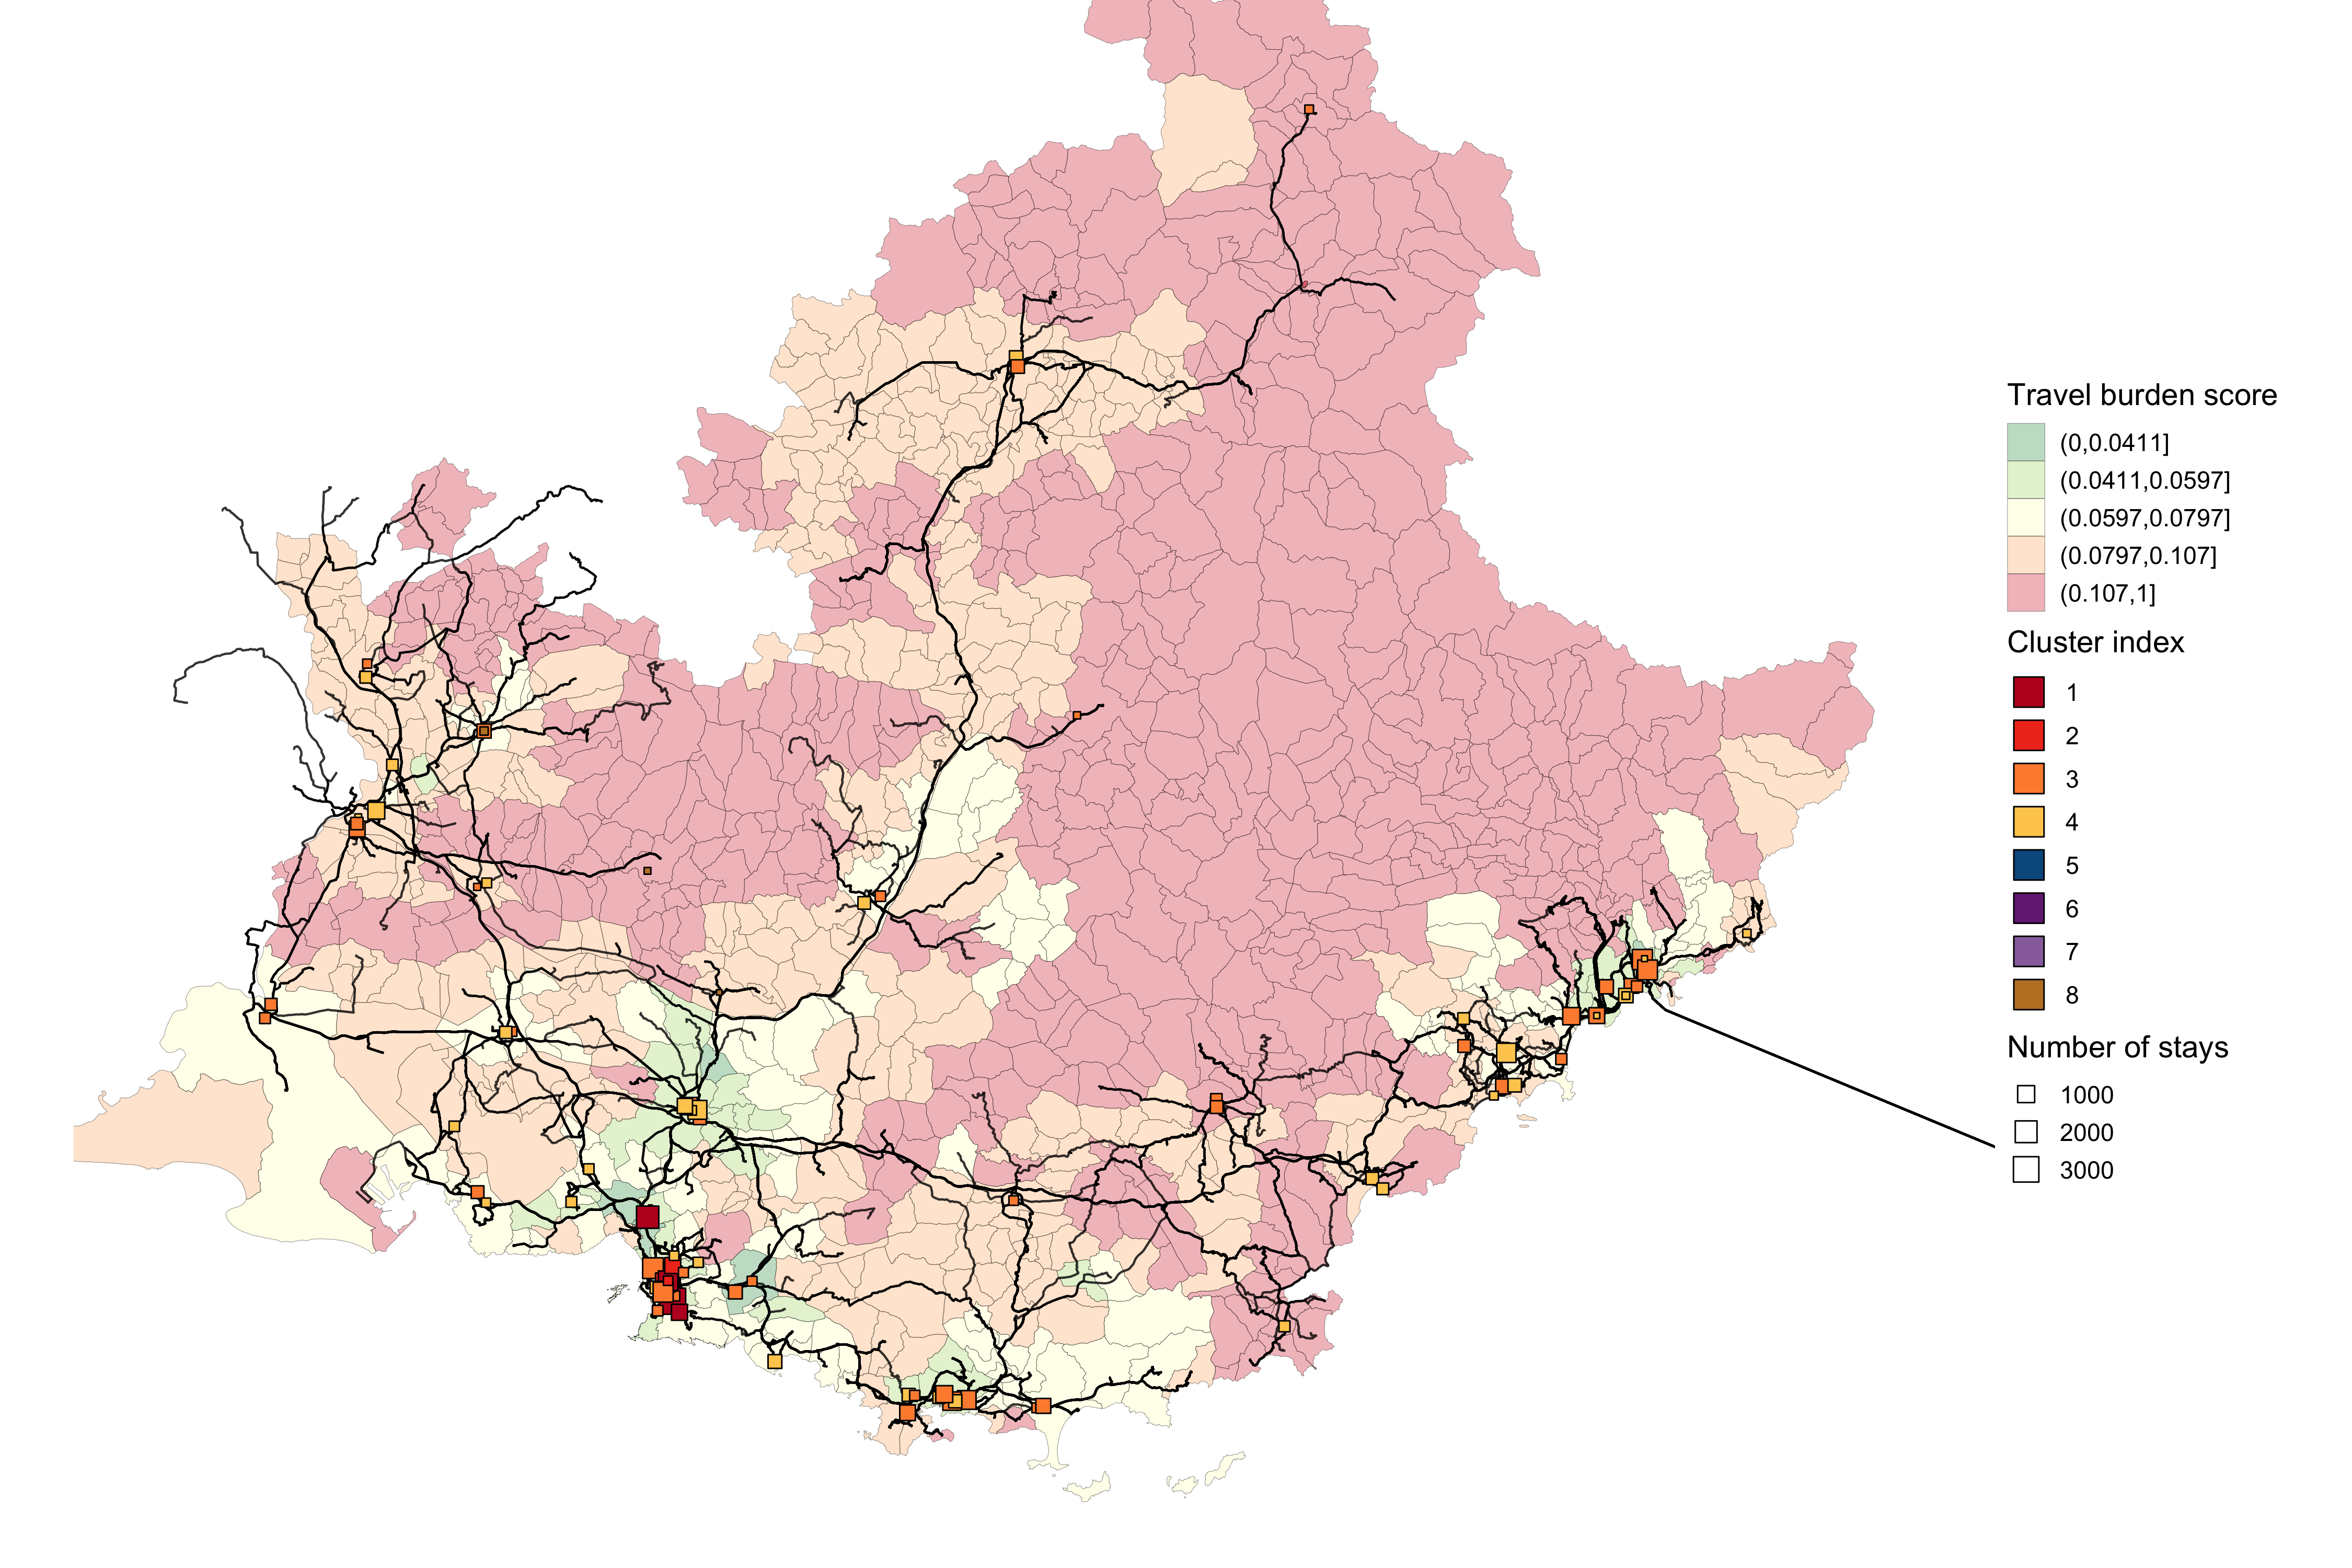
\includegraphics[width=0.9\textwidth]{images/routes/fig7.png}
    \centering
    \caption{
        \textbf{Travel burden score in Provence Alpes Cote d'Azur (PACA) region.}
        We compared the average travel burden score with the main roads
        location. The roads that with were used by less than 5 patients during
        the year are hidden. The areas that had low accessibility scores have
        high travel burden scores. However, we notice that some areas that had decent
        accessibility scores can have average or high average travel burden
        scores. This is probably due to the sinuosity of the roads, notably in
        the Var department, or in the north of Nice city. The roads in these
        areas are often small, with a lot of turns and roundabouts, increasing
        the travel tediousness. }
    \label{fig:travel-burden-paca}
\end{figure}

\subsection{Carbon footprint of patients travel}

We estimated the carbon footprint associated with patients' travels on
\cref{fig:routes-co2-emissions}. Since we only considered direct emissions, the
carbon footprint is proportional to the traveled distance. The alluvium chart on
sub-figure (A) displays the number of patients routes between municipalities on
the left and hospitals on the right, in the Ain department, located in
Auvergne-Rhone-Alpes region. This department mostly hosts rural municipalities.
The alluvium flows are sized by number of stays and colored by the stays carbon
footprint. The darker flows indicate higher \ac{co2} emissions. We point that
the routes with the more emissions are not necessarily the routes with the most
patients. To illustrate this, we focus on the Bourg-en-Bresse city, which is the
largest city from the Ain department. On plot (B) we show the total \ac{co2}
emissions per visited hospital, for patients living in Bourg-en-Bresse.
Centre-Hospitalier de Fleyriat is the most visit-ed hospitals among patients
living in Bourg-en-Bresse, with 150 stays and 4-kilometer distance between the
municipality centroid and the hospital. The resulting \ac{co2} emissions are 72
kg. However, some patients are traveling outside of Bourg-en-Bresse to reach
hospitals based in Lyon, which represents at least an 80 km drive. For instance,
there were 18 stays in Hospital Lyon Sud, located at 91 km from Bourg-en-Bresse.
The resulting \ac{co2} emissions were 184 kg, which is more than twice the
emissions of the 150 stays in CH Fleyriat.

\begin{figure}[h!]
    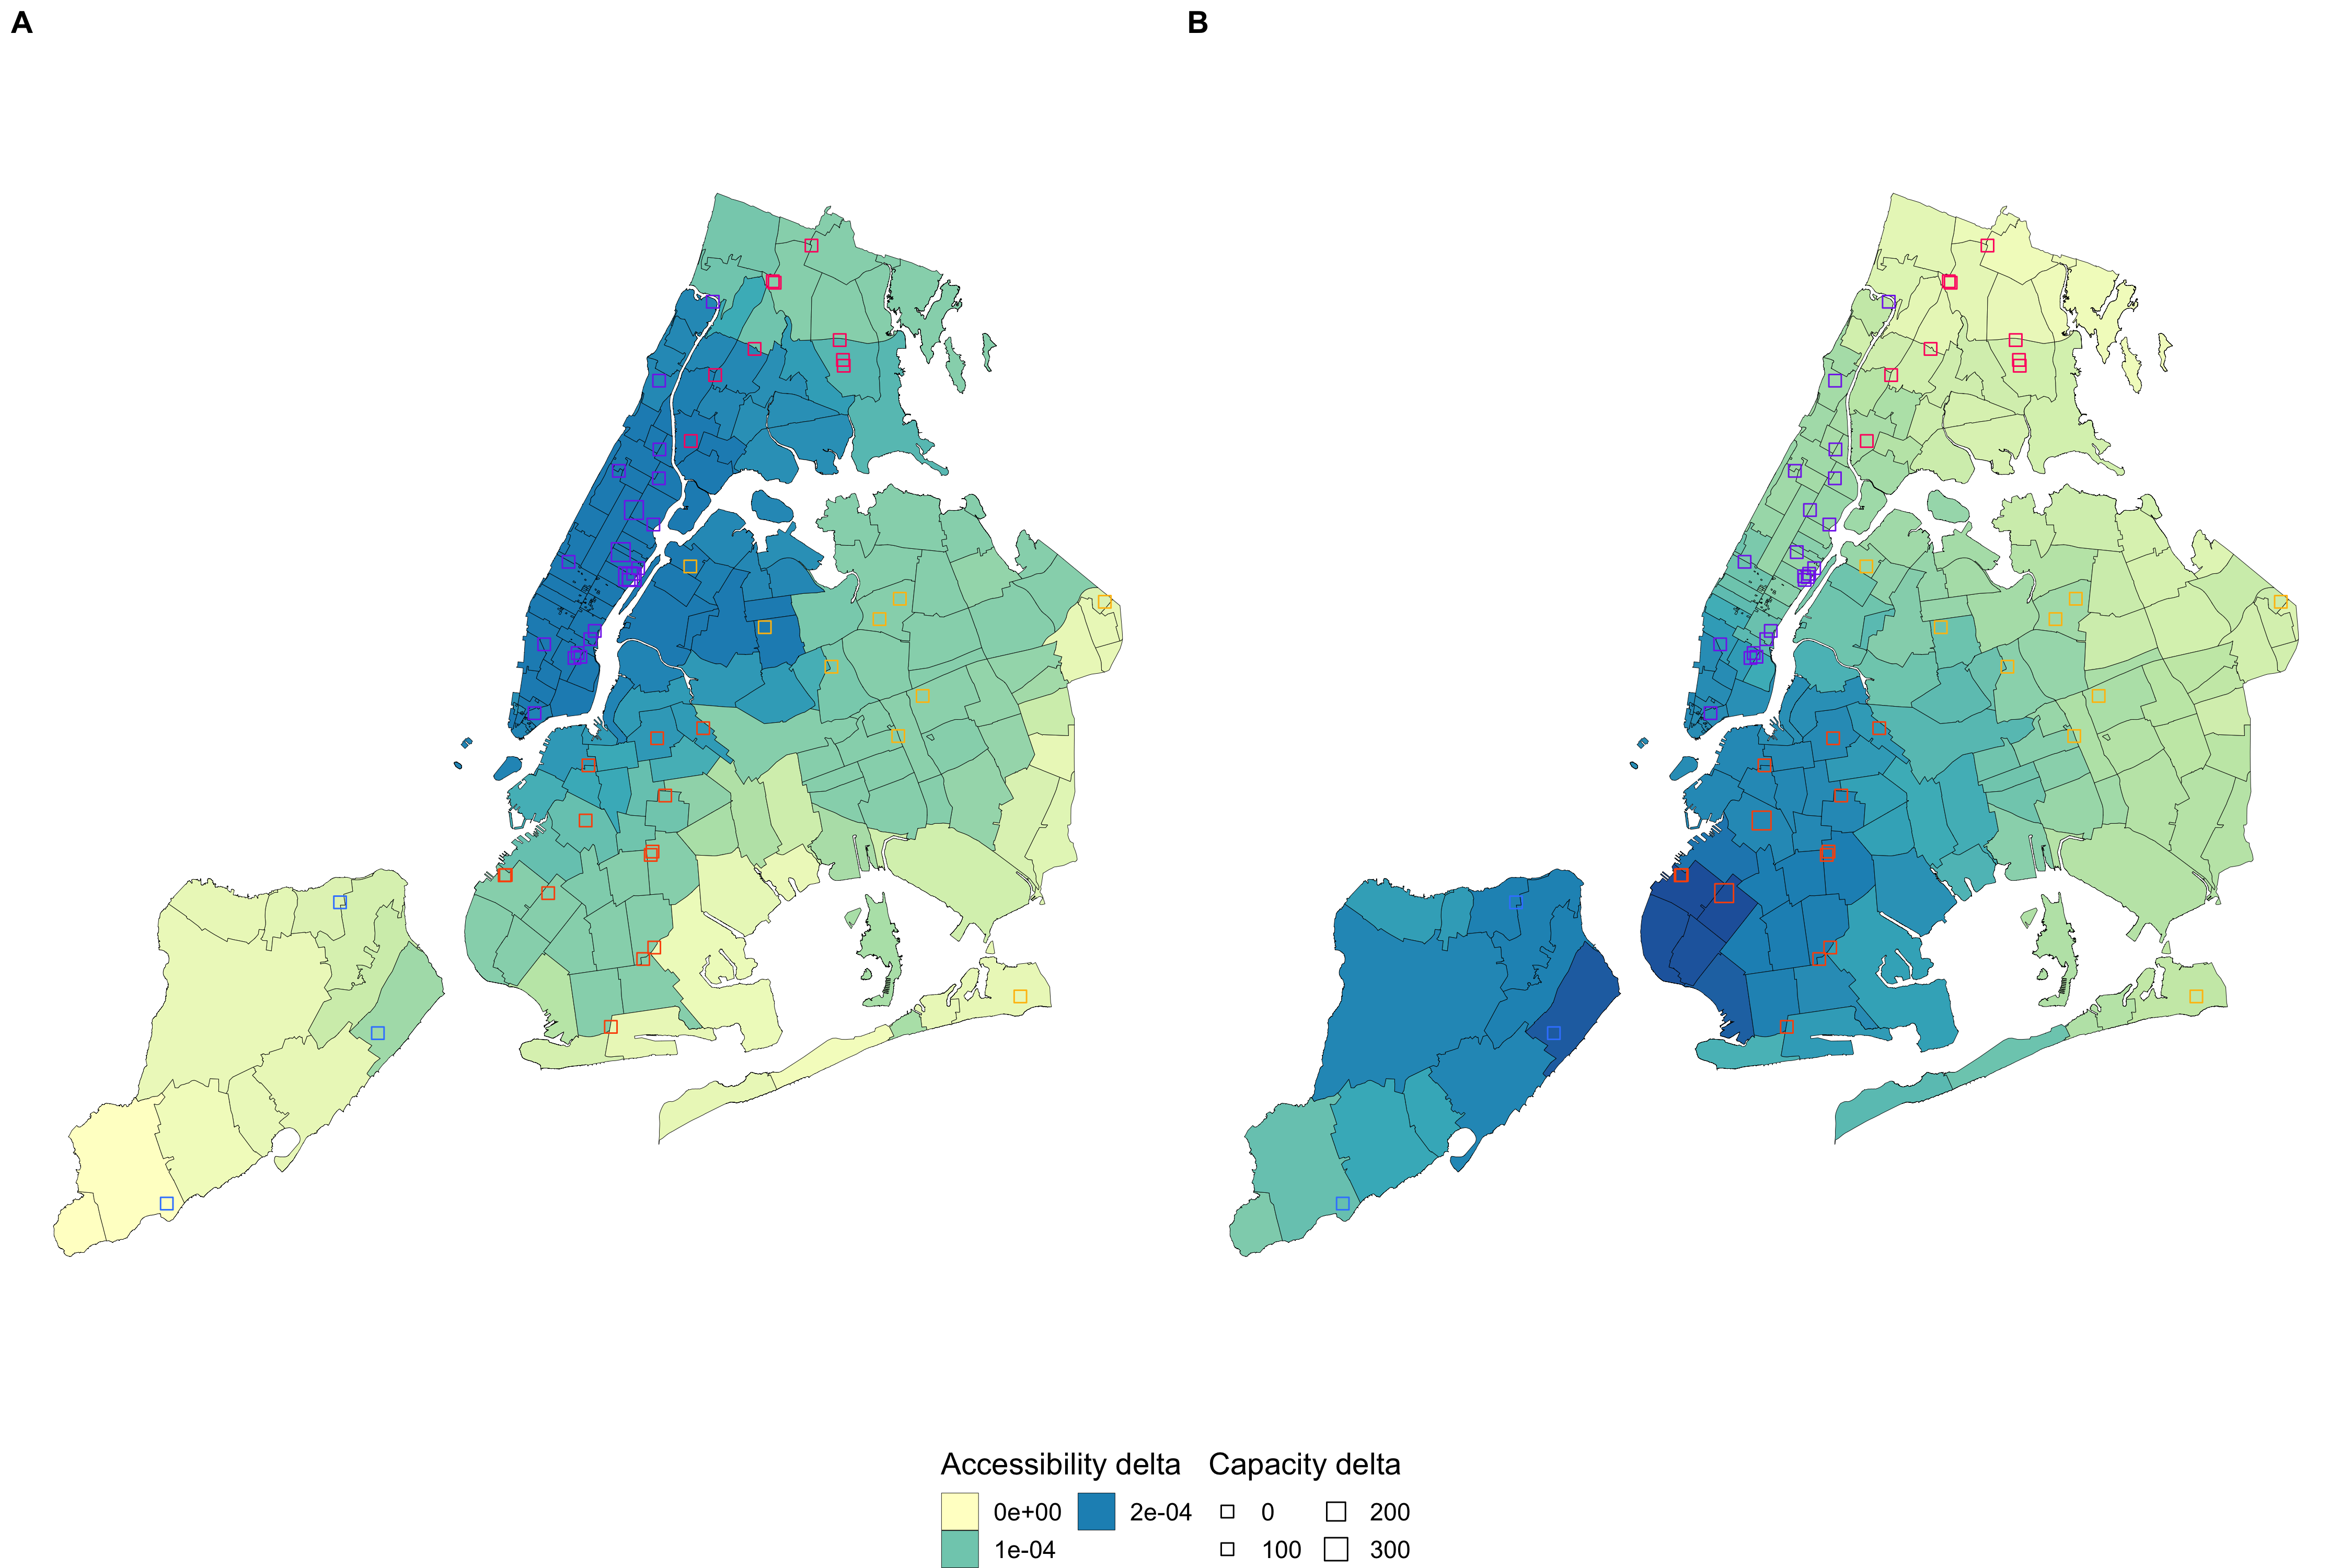
\includegraphics[width=0.9\textwidth]{images/routes/fig3.png}
    \centering
    \caption{ \textbf{\ac{co2} emissions for cancer patients travels} The
        \ac{co2} emissions are computed based on the GPS distance between the
        patient municipality centroid and hospital location. The total emission
        for a single travel is computed as the product of the average \ac{co2}
        emissions per km and the distance. Figure (A) displays the travels
        between municipalities in Ain department. Municipalities are on the
        left, hospitals on the right. Flows are sized by number of travels and
        colored by \ac{co2} emissions. Figure (B) shows the \ac{co2} emissions
        compared with number of stays in Bourg-en-Bresse city (Ain). The
        \ac{co2} emissions are higher for the fewer patients who traveled
        outside of the city to reach more specialized care centers in Lyon. }
    \label{fig:routes-co2-emissions}
\end{figure}

\subsection{Route optimization for cancer patients}

In this section, we present our results on patients route optimization, through
the Entropic Regularized Optimal Transport method. We recall that we aimed at
minimizing the distance traveled by patients, while making sure the hospitals
capacities were not exceeded. We included patients with breast cancer surgeries
stays, during the year 2018, in metropolitan France. This represented a total of
86,237 stays, between 5,456 population locations and 810 hospitals. The travel
distance matrix between the population locations and the hospitals was obtained
from the OpenRouteService API (\url{https://openrouteservice.org/}). We used the
\href{https://pythonot.github.io/gen_modules/ot.bregman.html#ot.bregman.sinkhorn}{ot.bregman.sinkhorn}
solver from ``POT: Python Optimal Transport'' \cite{flamary_pot_2021} to obtain
the \ac{ot} matrix with the optimal allocations.

The resulting allocations are displayed on \cref{fig:sinkhorn-distribution}. Map
(A) shows the allocations in Provence-Alpes-Cote-d'Azur region. Population
locations are displayed as blue triangles, sized by their populations. Hospitals
are displayed as red squares, sized by their capacities. Capacities have been
defined as the number of patients treated by the hospital within the year. The
black lines show the allocations between population locations and patients. The
line width is proportional to the number of patients sent from a population
location to an hospital. Since the algorithm minimized the traveled distance,
patients tend to visit the closer hospitals, while the capacity is not exceeded.
By comparing the number of patients by hospital before and after the
optimization algorithm, we noticed that the largest and most specialized
hospitals received less patients than before. These hospitals are often
saturated, and lowering the number of patients they receive could benefit them
as well as the patients treated there. These new vacancies could also be filled
by patients with more complicated cases or rare cancers that require a specific
expertise that not every hospital have. We are now interested in the global
effects of our optimization algorithm. Plot (B) displays the overall traveled
distance, and we notice that the optimization process nearly halved the overall
distance. The average traveled distance per patient went from 34.5 km to 21.9
km, a 36\% decrease. The overall carbon footprint similarly decreased from
293,009 tons of \ac{co2} to 186,141 tons of \ac{co2}. We compared the travel distance distribution before the optimization
(C) and after (D), and notice that very few patients travel further than 250
km with our method.

\begin{figure}[h!]
    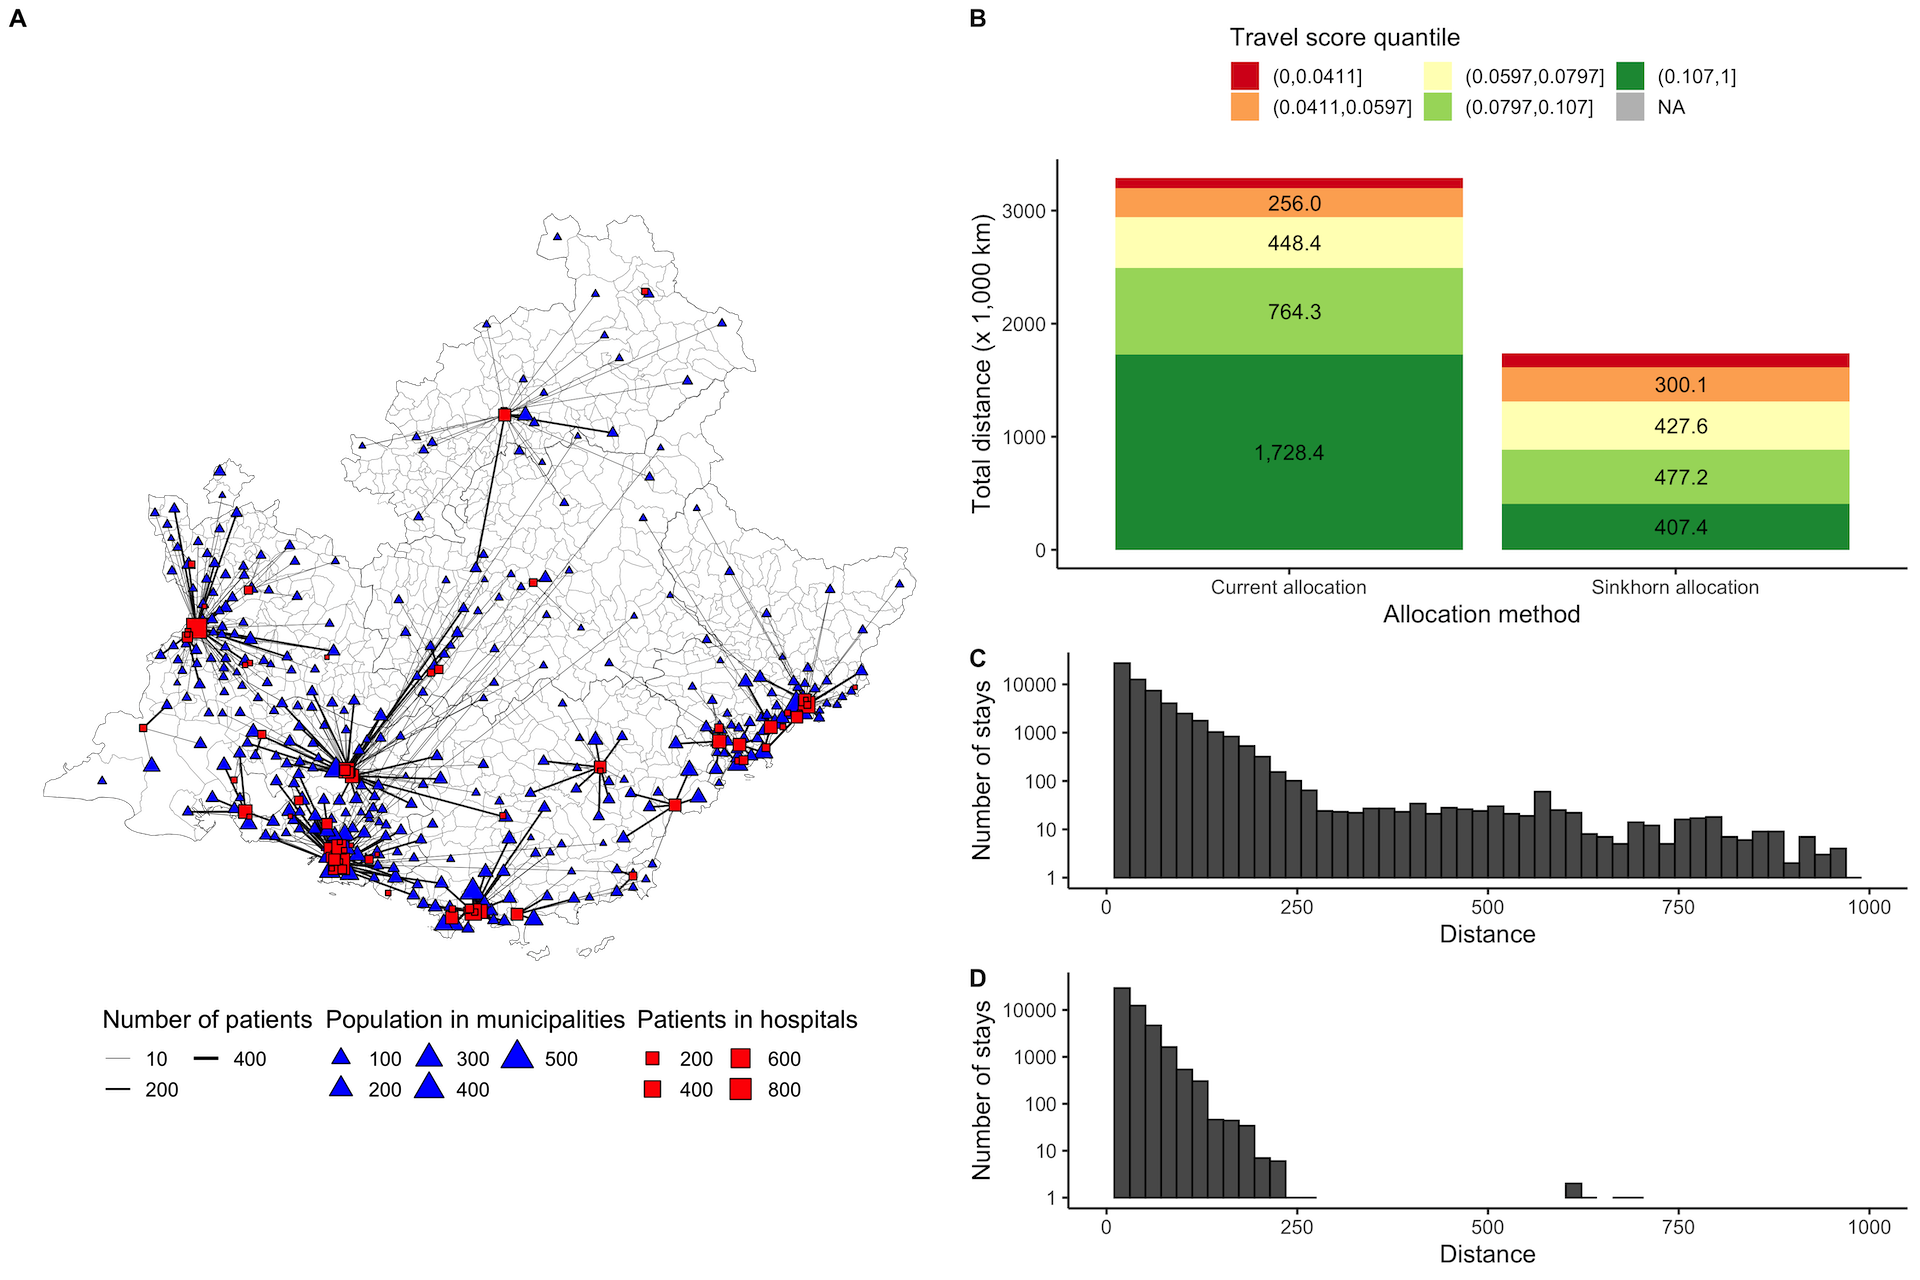
\includegraphics[width=0.9\textwidth]{images/routes/fig10.png}
    \centering
    \caption{ \textbf{Optimization results with the regularized Optimal
            Transport algorithm.} Map (A) shows the allocations in
        Provence-Alpes-Cote-d'Azur region. Population locations are displayed as
        blue triangles, sized by their populations. Hospitals are displayed as red
        squares, sized by their capacities. Plot (B) displays the overall traveled
        distance, and we notice that the optimization process nearly halved the
        overall distance. We compared the travel distance distribution before the optimization
        (C) and after (D), and notice that very few patients travel further than 250
        km with our method.}
    \label{fig:sinkhorn-distribution}
\end{figure}

The alluvial plots on \cref{fig:sinkhorn-alluvium} display the travels flux
between population locations on the right, and hospitals on the left, in the
Bouches du Rhone department (PACA region). The boxes are sized by the number of
patients living in the municipalities and treated in the hospital. The boxes are
sorted by decreasing number of patients. The paths are sized by the number of
patients who traveled from the population location to the hospital, and colored
by the travel burden quantile. The first alluvial plot on the left (A) displays
the routes before the optimization, and the second chart shows the new routing
after the \ac{ot} algorithm (B). Before the optimization process, the travel
burden scores were higher for municipalities with lower populations, i.e.
located to the bottom of the figure. We also notice that the proportion of
patients with more tedious travels is higher for the larger hospitals,
especially ``Institut Paoli-Calmettes'', which is the most specialized in
oncology care within the department. After the optimization algorithm was ran,
the proportion of patients with higher travel burden decreased. We also
notice that patients are routed more homogeneously. Indeed, patients within the
same municipality tend to be sent to the same hospitals.

\begin{figure}[h!]
    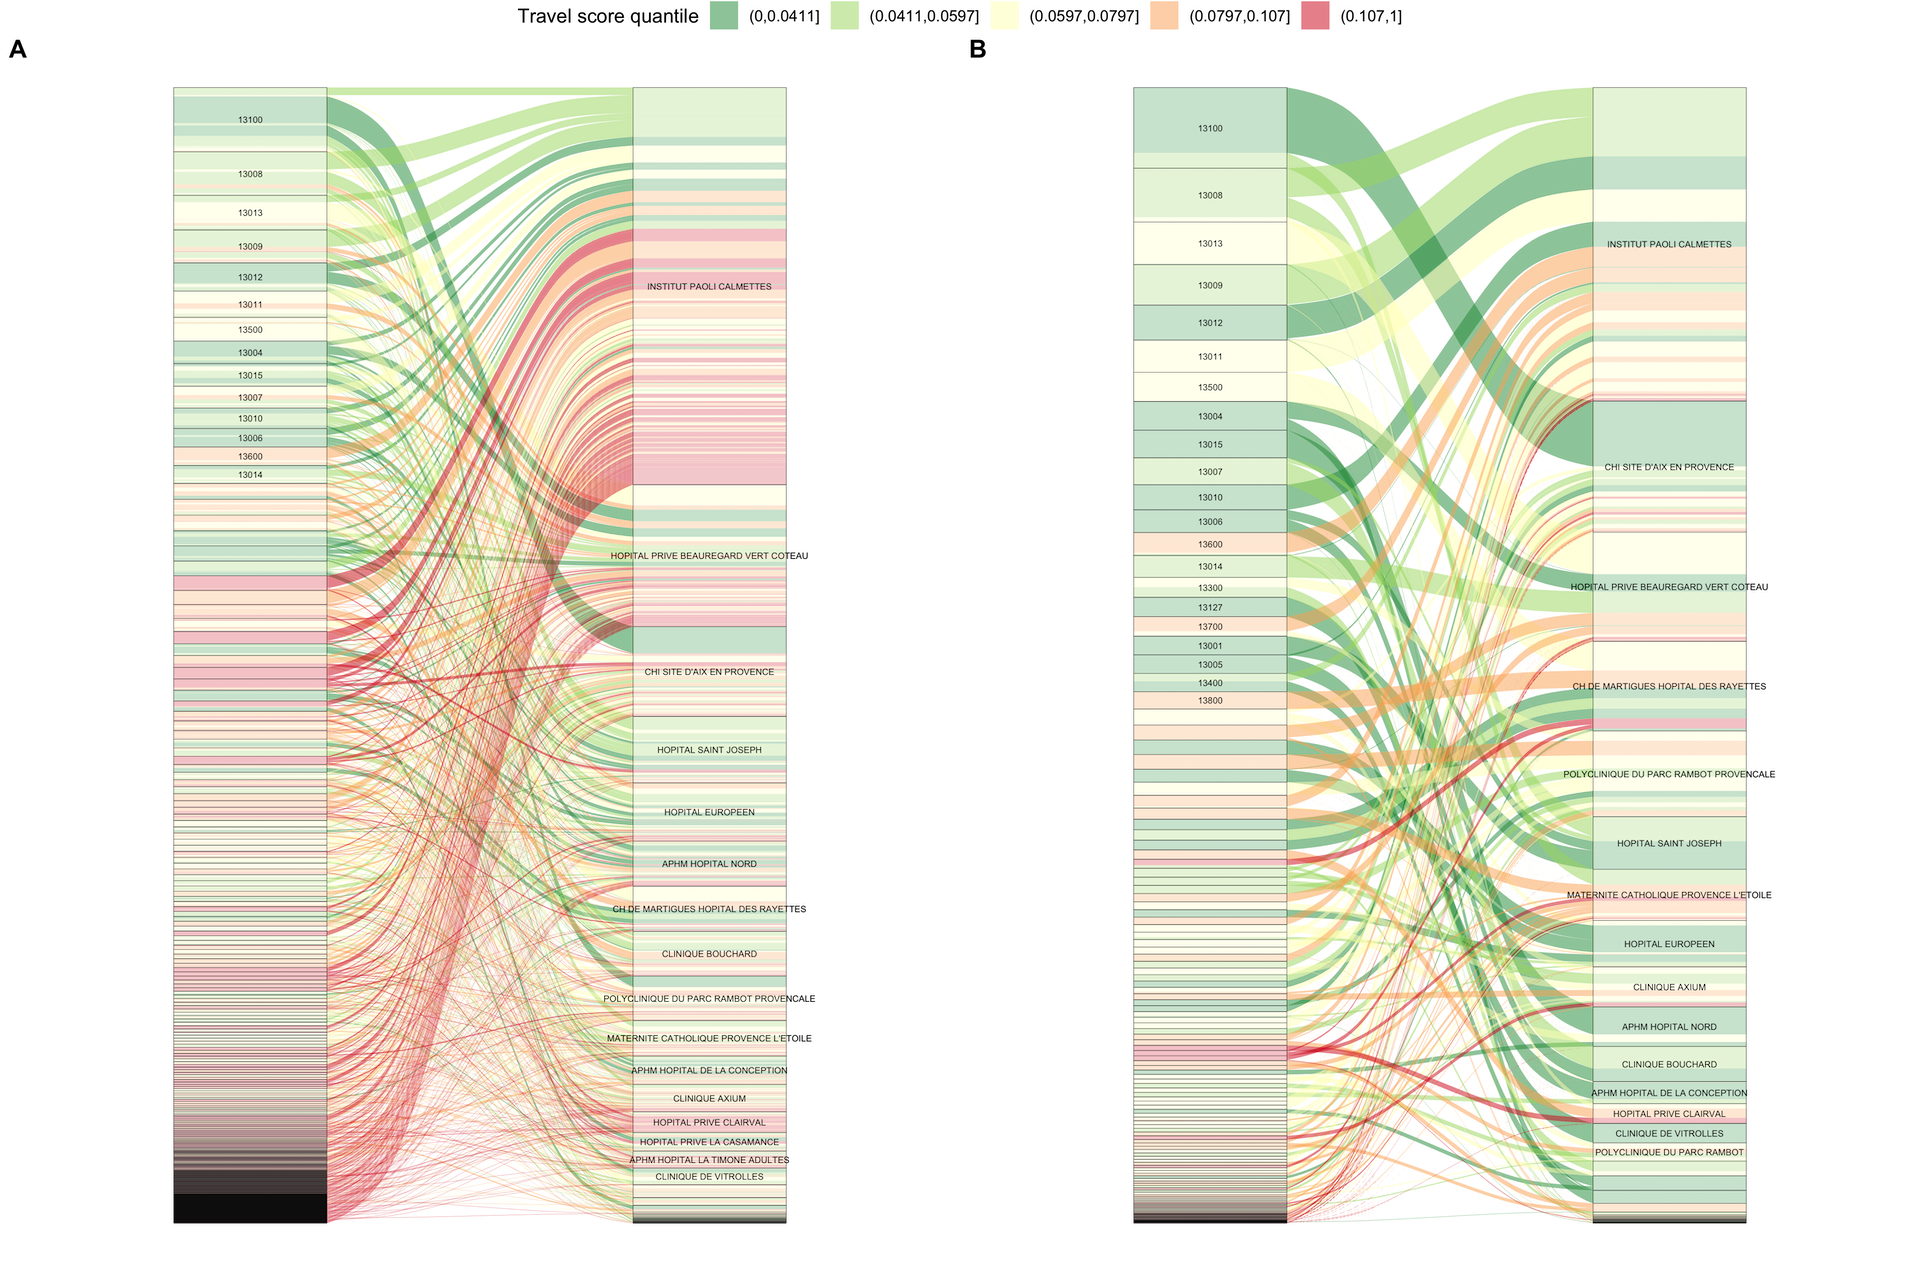
\includegraphics[width=0.9\textwidth]{images/routes/fig11.png}
    \centering
    \caption{ \textbf{Travel flux between in the Bouches du Rhone department
            (PACA region) before and after optimization.} The boxes are sized by
        the number of patients living in the municipalities and treated in
        the hospital. The boxes are sorted by decreasing number of patients.
        The paths are sized by the number of patients who traveled from the
        population location to the hospital, and colored by the travel
        burden quantile. The first alluvial plot on the left (A) displays
        the routes before the optimization, and the second chart shows the
        new routing after the \acf{ot} algorithm (B). }
    \label{fig:sinkhorn-alluvium}
\end{figure}

\section{Conclusion}

The results of the travel analysis for cancer patients in metropolitan France
concur with the effects of centralization of care observed in the literature.
We report longer travels for patients living in rural areas. The hospitals
specialized in oncology tend to receive patients from more distant population
locations. Finally, patients with less frequent cancers are forced to travel
further due to the limited number of hospitals that can correctly treat these
pathologies. We introduced the travel burden score, a new metric to consider
when studying patients travels. This score is proportional to not only distance
and duration, but also road sinuosity and number of roundabouts. The last two
variables, which are not explicitly captured by distance and duration, could be
responsible of more tedious drives for the patients, especially when their
health conditions are deprived. In our estimation, the \ac{co2} emissions are
directly proportional to the traveled distance. We did not consider indirect
emissions linked to the transportation. Car was the only transportation mean we
used, and we assumed every patient traveled by car, which might over-estimate
the \ac{co2} emissions. More research is needed to include public transportation
such as train or subway. The larger share of carbon emissions for cancer
surgeries is covered by frequent cancers, that can be treated in many hospitals,
like breast cancer for instance. For such pathologies, a rethink of the
centralization of care model might be needed. Patients from less dense
municipalities could be sent to closer regional hospitals if we make sure the
surgeons' expertise is good enough. Partnerships with larger and more
specialized hospitals could be created to spread the more up to date knowledge
outside the urban hospitals. However, this will be more complicated for rare
cancers, where expertise is scarce and concentrated in the larger hospitals. On
a carbon footprint perspective, we believe the lower number of concerned
patients makes it less of a priority. Finally, we simulated the case where
every patient would travel to the closest hospital, provided we do not
exceed the hospitals maximum capacities. We showed that the average driving
distance and \ac{co2} emissions were reduced by 36\%. While these results are
promising, only minimizing the traveled distance is not sufficient to
route the patients to the optimal hospital. More factors should be taken into
account, such as hospital specialization, quality of care, and detailed
patients characteristics. A tradeoff should be found between travel distance
and patient-hospital affinity. The case we presented where the patients
traveled to the nearest hospital is the most optimistic situation, and
despite this the driving distance and associated \ac{co2} emissions are
``only'' reduced by 36\%. Only considered surgery stays were considered here,
thus telemedicine will not be usable to reduce the footprint. The only lever
to reduce the associated carbon footprint is the average \ac{co2} consumption
of the driving vehicles, which will probably drop with the democratization of
the electric cars.
